\subsection{Objectives and ambition}

\label{sect:objectives}

As the values of \textbf{open science} and \textbf{reproducible science} are adopted by
governments, funding agencies, research institutes, and society,
there are practical challenges to implementing such practices on a global scale.

Two of the key societal goals of open science are facilitation of
\begin{compactitem}
\item \textbf{verification} of results, improving the reliability and trustworthiness of scientific output, and
\item \textbf{reuse} of research products, enabling commercial exploitation and/or derivative research.
\end{compactitem}

\noindent If results are merely \emph{available}, however,
much of the value of Open Science remains unrealised.
\myemph{Practical reproducibility} is required for efficient, widespread fulfilment of Open Science goals.
But what does it mean to be reproducible?
Without the \myemph{practical} ability to verify results, results are not
any more likely to be verified.
Without the \myemph{practical} ability to reuse work, results are not
any more likely to be exploited in new research or commercial work.

In \TheProject, we focus on ``practical reproducibility'',
specifically focusing on computational results, such as computer simulation, data
processing, data analysis, and creation of figures and tables in publications.
We differentiate ``technical reproducibility'',
where enough information is \emph{technically present} to reproduce the work given sufficient effort,
from ``practical reproducibility''
where effort to reproduce the work is not a burden~\cite{binder}.

\subsubsection{Ambition}

Computational reproducibility is a major challenge facing all scientific domains,
from social sciences to life sciences, physical sciences, engineering, and digital humanities.
Almost every area of academia must spend some time computing,
ranging from large-scale computer simulations to basic data analysis to produce a figure in a publication.

All of these face a common reproducibility challenge: \textbf{the computational environment},
or the collection of software used to produce the output.
To reproduce the work, a \textbf{sufficiently similar} computational environment must be produced to re-execute the code.
This may be a specific version of an application, or a large collection of software dependencies,
as is common in data science fields.

In order to meet the goals or policies of open and reproducible science,
\myemph{researchers need tools} to address the challenge. Ideally, those tools should
\begin{compactitem}
\item be freely available and open source (to maximise access and longevity); and
\item meet researchers where they are, as much as possible (to maximise practical adoption).
\end{compactitem}

\TheProject's main goal is to \myemph{improve the global reproducibility of
  scientific results} with a focus on those aspects of the research process that
are supported by computation and software, such as computer simulation, data
processing, data analysis and creation of figures and tables in publications.

We plan to achieve this goal through
\begin{compactitem}
\item educating researchers about good reproducible practices, and
\item making it easier to perform computational research in a reproducible way
  through improving and developing relevant software tools.
\end{compactitem}

Rather than re-inventing the wheel, we will build upon \textbf{existing tools and standards}.

Increasingly, open science and reproducibility are declared as values or requirements
at research institutions, governments, and funding agencies.
In order to meet these goals or requirements,
researchers need \myemph{tools} that help them accomplish the tasks required for reproducible work.

It is in this context that we set our objectives to \textbf{develop, experiment with, and mainstream Binder tools as concrete solutions and best-practices to increase the reproducibility of research}:

\begin{table}[H]
  \label{tab:objectives-tasks}
  \caption{
  Our objectives and their relationship to the work programme}
  \begin{tabular}{>{\raggedright}m{.2\textwidth}|m{.36\textwidth}|m{.36\textwidth}}

    \hline

    \myemph{Objective} & \myemph{Description} & \myemph{Relation to work programme}

    \\\hline

    \label{obj:reproducibility} Objective 1:\\\medskip \myemph{Evaluate and facilitate better computational
    reproducibility and FAIR data}
    &
    Tools for reproducibility must be evaluated by how successfully they produce the correct environment.
    We will provide evaluation tools for reproducibility,
    and use these tools to guide improvements to the Binder tools,
    solving known issues where we can improve the \myemph{reproducibility of computational environments}
    used for science, and facilitate \myemph{FAIR data practices}.
    &
    The core of this effort is to \textbf{develop, validate, pilot, and deploy practices and practical tools for funders, publishers, and scientists}.
    The robustness of these tools is key to their utility and value,
    and thereby adoption in research communities.
    \\\hline

    \label{obj:broaden} Objective 2:\\\medskip
    \myemph{Enable reproducibility using common tools in a wider variety of environments}
    &
    We develop \textbf{generic tools for reproducible software environments},
    but have identified several areas where the Binder tools do not yet meet user needs,
    such as traditional \textbf{HPC environments}, or users with \textbf{large data sets}.
    We shall address those gaps so that tools and strategies can be shared by a wider variety of communities,
    aligning effort and reducing necessary duplication.
    &
    In order to \textbf{promote uptake, greater collaboration, and increased alignment of the activities of stakeholders},
    it is most efficient when knowledge and tools can be shared.
    When tools do not work for significant fractions of the research community,
    they must develop their own, often similar tools,
    as has often been the case for the HPC community.

    \\\hline

    \label{obj:demonstrators} Objective 3:\\\medskip
    \myemph{Demonstrate reproducibility in specific scientific applications}
    &
    We will demonstrate the utility of the Binder tools for achieving reproducible research
    in a variety of scientific domains,
    which serves both to \textbf{inform and motivate} improvements to the system,
    and as \textbf{illustration and reference} for others to follow.
    &
    By collaborating across domains, we \textbf{promote uptake, greater collaboration, and increased alignment of the activities of stakeholders}.
    Further, by publishing working examples,
    we contribute to an \textbf{open knowledge base of results, methodologies and interventions on the drivers and consequences of reproducibility} in these specific domains,
    to be used as reference or followed by others in the same domain
    and other domains with similar challenges.

    \\\hline

    \label{obj:education} Objective 4:\\\medskip
    \myemph{Educate researchers about reproducible practices}
    &
    Develop \textbf{best practice guidelines} for reproducible science, and disseminate this by
    \textbf{educating the research communities} about reproducible practices and available
    tools for reproducible publications and policies. \textbf{Reach out} to scientists, and
    the wider research communities and reproducibility stakeholders to encourage
    engagement with this project.
    &
    By collecting expertise and guidelines, we contribute an \textbf{open knowledge base of results, methodologies and interventions}
    for computational reproducibility.
    \\\hline

  \end{tabular}
\end{table}

\subsubsection{Binder tools for reproducible research}
\label{sec:reproducibility-example}

Binder\footnote{\url{https://jupyter.org/binder}} is a project providing open source tools to solve this computational environment reproducibility challenge.
It has already proven useful for at least tens of thousands of researchers, educators, developers, and students,
and we believe it has the potential to \textbf{facilitate practical reproducibility for millions} more,
including in institutions, funding agencies, and policy makers.
We aim to realise that potential by extending Binder open source tools.

\begin{figure}[htb]\centering
  \includegraphics[width=0.9\textwidth]{use-cases-binder-logbook-solution.png}
  \caption{A typical use case for Binder-based reproducibility using Jupyter notebooks in research.
            Image by Juliette Belin for the OpenDreamKit project, used under
            CC-BY-SA.}\label{fig:use-cases-binder}
\end{figure}

We start with an example making use of existing \textbf{Binder
tools for computational reproducibility}. Starting from this base-line, we can
explain what progress and additional impact we will enable through this project.

Figure~\ref{fig:use-cases-binder} depicts how a scientist can use a Jupyter
notebook and the Binder software to make her research results easily
reproducible and reusable. Jupyter notebooks are popular with millions of researchers and allow the creation of notebook
documents, containing a mixture of text and interactively executable code, along with rich output from
running that code. In short:
\begin{compactitem}
\item Scientist Jane has created a \myemph{notebook that carries out computations} or
  data processing and creates a figure based on those results. For the purpose
  of the introduction of this workflow, we assume that
  Figure~\ref{fig:reproducibility-example-covid} shows this figure.

\item She has made the notebook and raw data available in a \myemph{public repository}
  (for our example at\newline
  \mbox{\url{https://github.com/fangohr/reproducibility-repository-example}}).

\item As she has described \textbf{what software is needed} to execute her notebook (more
  details below), it is possible for all interested scientists (and anybody
  else, including the reviewers of this proposal) to \myemph{reproduce} her
  figure.

  To reproduce the figure, one needs to visit an online URL\footnote{\url{https://mybinder.org/v2/gh/fangohr/reproducibility-repository-example/HEAD?labpath=figure1.ipynb}}
  (combination of the public repository and online Binder service) in a browser, and then wait a minute or so for a dedicated computational
  environment to be created and started. Then select 'Run' -> 'Run all cells'
  from the menu of the interactive Jupyter notebook that will appear in the
  browser.

  At that point, the computational steps that Jane has carried out to create her
  result are repeated, and the results are \myemph{reproduced}.

\item Because all the computational steps are captured in the Jupyter notebook,
  they can be inspected and interrogated if desired. In particular, the steps
  can be modified and re-executed: this allows very efficient \myemph{re-use} of
  the results by other researchers.
\end{compactitem}

We provide a more detailed description of the components and steps in this
process in the following sections \ref{sec:opensource}.

The reproducibility workflow shown in Figure~\ref{fig:use-cases-binder} is
working today, and we provide estimates on the number of current users in
section \ref{sec:mybinder}. The work proposed for this project will build on
this existing technology and (i)~make it \myemph{more robust and easier to use}
(\WPref{reproducibility}), and (ii)~extend the functionality (\WPref{impact}) so
that the existing tools can be \textbf{used in many more use cases}
(\WPref{applications}).

We note in particular that the Binder-enabled workflow for reproducibility has
originally been developed to reproduce results that are created within Jupyter
notebook (as shown in Figure~\ref{fig:use-cases-binder}).
However, the approach taken is generic, and not specific to notebooks: it is
based on \repotodocker (Section~\ref{sec:repo2docker}), a tool to \textbf{build, run, and
publish} Docker images from source code repositories.
As part of this project, we will demonstrate that reproducible
computational environments can be created using the same approach
in studies that do not make use of Jupyter notebooks.

\begin{figure}
  \centering
  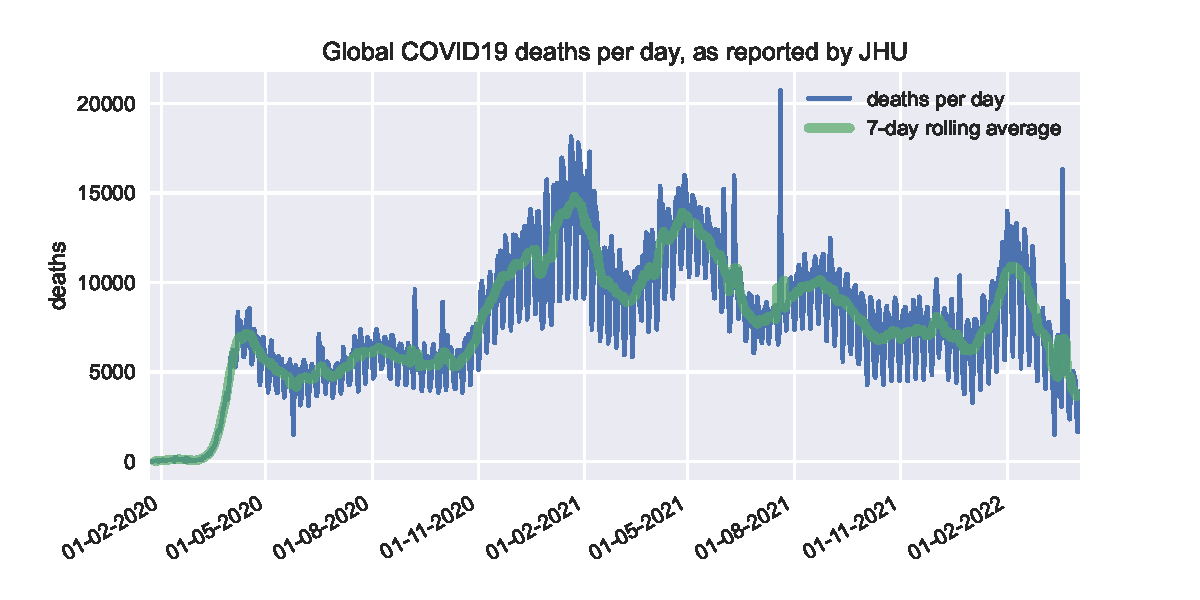
\includegraphics[width=0.8\textwidth]{images/figure1.pdf}
  \caption{Figure (\softwarename{figure1.pdf}) which can be reproduced in our explanatory repository example
    \cite{ReproducibilityRepositoryExample2022}. \label{fig:reproducibility-example-covid}}
\end{figure}


\subsubsection{State of the art}

To make computational research \textbf{reproducible}, we generally need to make available
(i)~required \textbf{data}, (ii)~the required \textbf{software}, (iii)~the \textbf{protocol} that explains
how to process the data to obtain the result that is to be reproduced. Using
services such as Zenodo, it is possible to deposit such archives with a DOI and
make reference to them in publications.

In order to reproduce the results, it should be possible for anybody to take such an archive of a research
output, and to carry out the two necessary steps:
\begin{compactitem}
\item Step 1 to install the required software, and
\item Step 2 to follow the protocol to reproduce the results from the archived data.
\end{compactitem}

It is of particular value if Steps 1 \emph{and} 2 can be \emph{carried out
  automatically} by executing a program included included in the
archive. First, if the automatic execution is possible, we know that there is a
complete description of the protocol included in the archive, and that no
mistake is made in trying to follow the protocol. Second, the automatic
execution saves time.

There are two common approaches to achieve this reproducibility: (a) to use a
\textbf{workflow} tool or environment that caters to a given use case (for example
~\cite{reana2019} ~\cite{Afgan2018} ~\cite{Mlder2021})
and encapsulates the full process for strong reproducibility guarantees.
Or (b) to use \textbf{standard} (software engineering) \textbf{computing tools} and conventions
(git, make, python, perl, bash, \ldots)
to specify the compute environment and reproduce steps piecemeal.

The workflow tool approach (a) is robust, but requires `all-in' adoption by authors and reproducers alike,
and is \textbf{difficult in practice}. It can also have associated `vendor lock-in' effects
- once a tool is adopted for one piece, it must be used for all associated work.
A consequence of this more tailored approach is \textbf{reduced re-use and duplication of effort}.
As a workflow tool may not meet the needs of a community,
that community must then build its own tool, or be left \textbf{without appropriate tools}
if they lack the resources or expertise to build their own.
Workflow tools also often \emph{dictate} a significant amount of how researchers perform their work,
which can inhibit adoption when it does not suit their existing patterns.

The \textbf{standard computing tools} approach (b) is generic, but \textbf{not accessible} to all researchers
as it requires substantial training or experience to be effective,
and it is prone to errors or incompleteness when executed,
leading to the "Works for Me" problem,
where the author may have no trouble reproducing their own work,
but they have not effectively communicated the requirements such that others can do the same.
The \textbf{gap between researchers' expertise and practical need} when it comes to these tools has led to the creation
of whole industries of remedial skills training.
The loose coupling of tools and modular choices make it \textbf{more flexible} (covering more use cases),
but \textbf{more difficult} to follow robustly.
Identifying which tools to use and following appropriate installation is a challenge
for both authors, who must communicate requirements clearly without knowing the reader's context,
and readers, who must find, understand, and follow potentially complex directions, even assuming they were
complete and correct.

\medskip Researchers who use the Jupyter notebook to orchestrate their
computational research can achieve this automatic
reproducibility with little additional effort~\cite{Beg2021}: they use the notebook document as
the protocol of their analysis (Step 2), which can be executed automatically.
They can make use of the \textbf{Binder tools} (Section~\ref{sec:opensource}) and/or the
associated  mybinder.org\footnote{\url{https://mybinder.org/}} service (free and public) that has
been designed by the Jupyter team to \textbf{automatically create the appropriate
software environment} (step 1) in which the notebook can be executed.

BinderHub instances such as mybinder.org are extremely convenient,
but being hosted services they do not offer the autonomy
of private execution on one's own computational resources,
be they a local machine or cloud or on-premises clusters.

\subsubsection{Beyond the state of the art}

In this project, we will focus on the \myemph{reproduction of the
software environment} (Step 1) which is a prerequisite for any attempt to
reproduce the actual research outputs. In particular, we want to make the
creation of this computational environment \myemph{automatic}, \myemph{generic} and \myemph{robust},
especially for long-term preservation.

We will go beyond the current state of the art by bringing the following selected improvements:
\begin{compactitem}
\item Currently, producing valid computational environments from published scientific publications and/or existing
      online repositories is difficult and usually requires manual handling of the process which is cumbersome and
      time consuming. \textbf{Improving the robustness of Binder tools} and in particular \repotodocker{}'s ability to
      produce computational environments, long after the publication and/or release,
      through testing and development, as well as taking additional context information into account,
      such as repository publication date, will enable \textbf{seamless reproduction of computational environments};
\item The existing \textbf{Binder tools} are already widely used in the Jupyter user community,
      but the focus has been on the reproducibility of Jupyter notebooks that may not fit everyone’s needs:
      for instance mastering one of the many programming languages (> 40) supported by Jupyter is required and limits take-up by some communities.
      Highlighting and extending \textbf{Binder tools}' \textbf{capabilities beyond notebooks}
      will undoubtedly \textbf{attract new communities} of users and can facilitate
      \textbf{transfer of knowledge} between academia and industry;
\item The current \textbf{Binder tools} rely on Kubernetes and deploying a Binder service requires technical skills that are
      beyond many institutional or companies IT support staff. As a result, most researchers rely on existing
      deployments that are overloaded and cannot cope with the huge demand, and they may disregard Binder
      as a viable solution for creating reproducible computational environments. Being able to use \repotodocker{}
      anywhere e.g. from the user’s personal laptop (Binder@Home, \taskref{applications}{binder-at-home}) to the
      most powerful supercomputers (Binder@HPC, \taskref{applications}{binder-at-hpc})
      by removing technical restrictions such as the dependence on Kubernetes,
      and supporting a wider variety of community practices for reproducible environments
      will open new ways of using Binder tools that are more in line with the current needs of end-users;
\item Another important bottleneck is the need to \textbf{access and to reuse very large and complex datasets} (sometimes
      with restricted access permissions) that are published and deposited on (domain-) specific long-term archives.
      Specific use cases (to read and process such datasets) are provided by end-users (either as part of the dataset
      itself or separately) but the usage of the Binder software and/or existing public Binder deployments for
      this use case is not yet well supported (such amount of data cannot be easily and efficiently moved to
      public Binder instances).
      \emph{Ad hoc} or domain-specific solutions (for instance the usage of cloud optimized
      data formats and associated catalogs such as intake\footnote{https://intake.readthedocs.io/en/latest/index.html}
      or STAC\footnote{https://stacspec.org/} by the Pangeo\footnote{https://pangeo.io/} Geoscience community)
      have been explored by diverse communities but are technically difficult and not generic enough to be
      adopted by everyone. The Binder software will be extended to \textbf{facilitate data publishing} (see \taskref{applications}{data-publishing}) with
      the plugin of external long-term archive resources and enable the \textbf{publication and reuse of large and complex datasets}.
\end{compactitem}


\subsubsection{Motivation - why?}\label{sec:motivation-why}

We focus on the \textbf{computational reproducibility} because it is a real
obstacle for \textbf{practical reproducibility}.

First, it affects the majority of all researchers: there are estimates that \textbf{over
92\% of all researchers} work with research software and over 50\% develop
their own~\cite{Hettrick2014}. Where experiments drive the research, this is
often data processing, analysis, and plotting. Each of those computational
research cases needs a \textbf{software environment} in which the actual processing can
be carried out. The software environment may consist of somewhat standard
packages (for example use of a Python, R, or Julia plotting library), or it may
include tailored programs that have been developed specifically for a study.

Second, software packaging and management is a technically challenging topic,
and \textbf{we cannot expect 92\% of all researchers to master it} -- so we believe there
is a clear need to support them with appropriate tooling.

The complexity arises in parts from the increasing age of archived studies, and
also in the often unusual combinations of research software and libraries that
need to be combined for a particular study. Other difficulties include that a
reproduction typically needs to be done on a different computer, perhaps even on
a different operating system. If, say, a plotting library is used, then it may
change its interface or behaviour over time, so it is important to install
exactly the right version of the plotting library, before a reproduction of
results is attempted using it.

Third, being able to recreate the appropriate software environment is a
prerequisite before any actual reproduction of results can be attempted: it
would be inefficient to educate researchers what data and programs to archive,
if in the future nobody (or only very few highly trained people) will be able to
execute those scripts.

Finally, we think that there are low-hanging fruits: the work proposed here will
make it possible to create computational environments automatically for
\myemph{existing data archives}: the Binder philosophy is to support existing standards for software
specification, and to \myemph{automatically} build a software environment based on those standards.
Where researchers have used the existing software specification already, Binder tools
will work immediately on their archived files. This means that (i)~a researcher
putting together a well-organised archive does not need to know about Binder tools,
yet the researcher who wants to reproduce the results later can use Binder tools to
automate the recreation of the software environment. This also means that
(ii)~improvements we propose in this work, will make some existing archives (that
have been created in the past) more easily reproducible.
To reiterate: \textbf{researchers do not need to use Binder tools to benefit}.

%(It is part of our training programme to educate about the importance and methods
%for software specification.)
